\documentclass[slidestop, mathserif]{beamer}

% \mode<presentation>
% {
% 	\usetheme{Warsaw}
% 	\setbeamercovered{transparent}
% }

\usepackage{caption}
\usepackage{subcaption}


\mode<presentation>{
	\usetheme{Berlin}
	\setbeamercovered{transparent}
	\usefonttheme{professionalfonts}
}

\usepackage{amsmath, amsfonts, amssymb}
\usepackage{mathrsfs,dsfont}

\newcommand{\norm}[1]{\left\|#1\right\|}
\newcommand{\suchthat}{-\hspace{-10pt}\ni\hspace{-10pt}-}


\AtBeginSection[]
{
   \begin{frame}
       \tableofcontents[currentsection]
   \end{frame}
}

%% want to use verbatim: \begin{frame}[fragile]

\title[Metrics for Tracking]{Metrics for Trackings: Evaluations and Comparisons}
\author[chy1010]{Chien, Hung-Yu (chy1010) \\ {\tt andy1010@gmail.com}}
\date{\today}

\begin{document}

\begin{frame}
    \titlepage
\end{frame}

% \section[Outline]{}
% \begin{frame}
%     \frametitle{Outlines}
%     \tableofcontents
% \end{frame}

\section{Preliminaries}

\begin{frame}
	\frametitle{MOT (Multiple Object Tracking)}

	Given a video, the task of MOT consists of the following parts:
	\begin{itemize}
		\item locating multiple objects,
		\item maintaining their identities, and
		\item yielding their individual trajectories.
	\end{itemize}

    In more details, each object is assigned a unique id in a frame.
    And objects with the same id in consecutive frames form a trajectory.

    \begin{figure}
        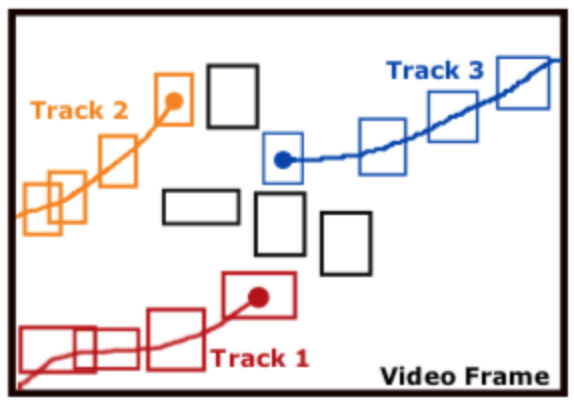
\includegraphics[height=70pt]{pics/fig1.png}
        \caption{objects with the same id from different frames}
    \end{figure}

\end{frame}

\begin{frame}
    \frametitle{Matching in Frame-Levels}

    Here a {\bf matching} is a \emph{1-1 relation} between ground-truths
    and predictions in the same frame.
    It can be done by according to the {\bf similarities} of every `gt-pred' pair.
    For example, $\max\{1-\text{\tt dist}, 0\}$ and {\tt IoU} are metrics for
    measuring similarity, which is in $[0,1]$.

    \vspace{4pt}

    Denote $\mathcal S(g_i, p_j)$ be the similarity score of $i$-th ground-truth object
    and $j$-th prediction. Let $\alpha\in(0,1)$.
    Then a matching $\Pi$ under the similarity threshold $\alpha$ is a 1-1 relation
    satisfying
    \[
        (g,p) \in \Pi \Rightarrow \mathcal S(g, p) \geq \alpha. ~ \text{($g$, $p$ must belong the same frame.)}
    \]

    % \vspace{2pt}

    \emph{1-1 relation: if $(g_i, p_j)$, $(g_k, p_\ell)\in \Pi$,
    then $i=k$ $\Leftrightarrow$ $j=\ell$.}

\end{frame}

\begin{frame}
    \frametitle{Trivial Notions}

    Denote $F:=\{f_0, f_1, \ldots, f_{N-1}\}$ as the set of frames.
    If $\Pi$ is a matching, it can be a matching inside a frame $f$ and specified by $\Pi^{(f)}$;
    or be a matching in all frames.
    When $\Pi$ denotes a global matching, it is the union of all its sections:
    $\Pi = \cup_{f\in F}\Pi^{(f)}$.

    \vspace{4pt}

    Furthermore, once a collection $E$ is defined globally,
    we denote $E^{(f)}$ as the $f$-section, i.e. elements inside frame $f$.

    \vspace{4pt}

    For a ground-truths $g$ or a prediction $p$, denote
    \begin{itemize}
    \item $f_g$ / $f_p$ as the frame it appears;
    \item $\text{gtId}(g)$ / $\text{prId}(p)$ as its id;
    \item $\text{gtTr}(g)$ / $\text{prTr}(p)$ as its trajectory (objects with the same id).
    \end{itemize}
\end{frame}

\begin{frame}
    \frametitle{TP, FP and FN}

    For a given matching $\Pi$ during all frames, we can define:
    \begin{itemize} \itemsep = 2pt
    \item TP, $\text{TP}_\Pi$ (true positive cases): Matched pairs in $\Pi$.
    \item FP, $\text{FP}_\Pi$ (false positive cases): Non-matched predictions.
    \item FN, $\text{FN}_\Pi$ (false negative cases): Non-matched ground-truths.
    \end{itemize}

    \begin{figure}
        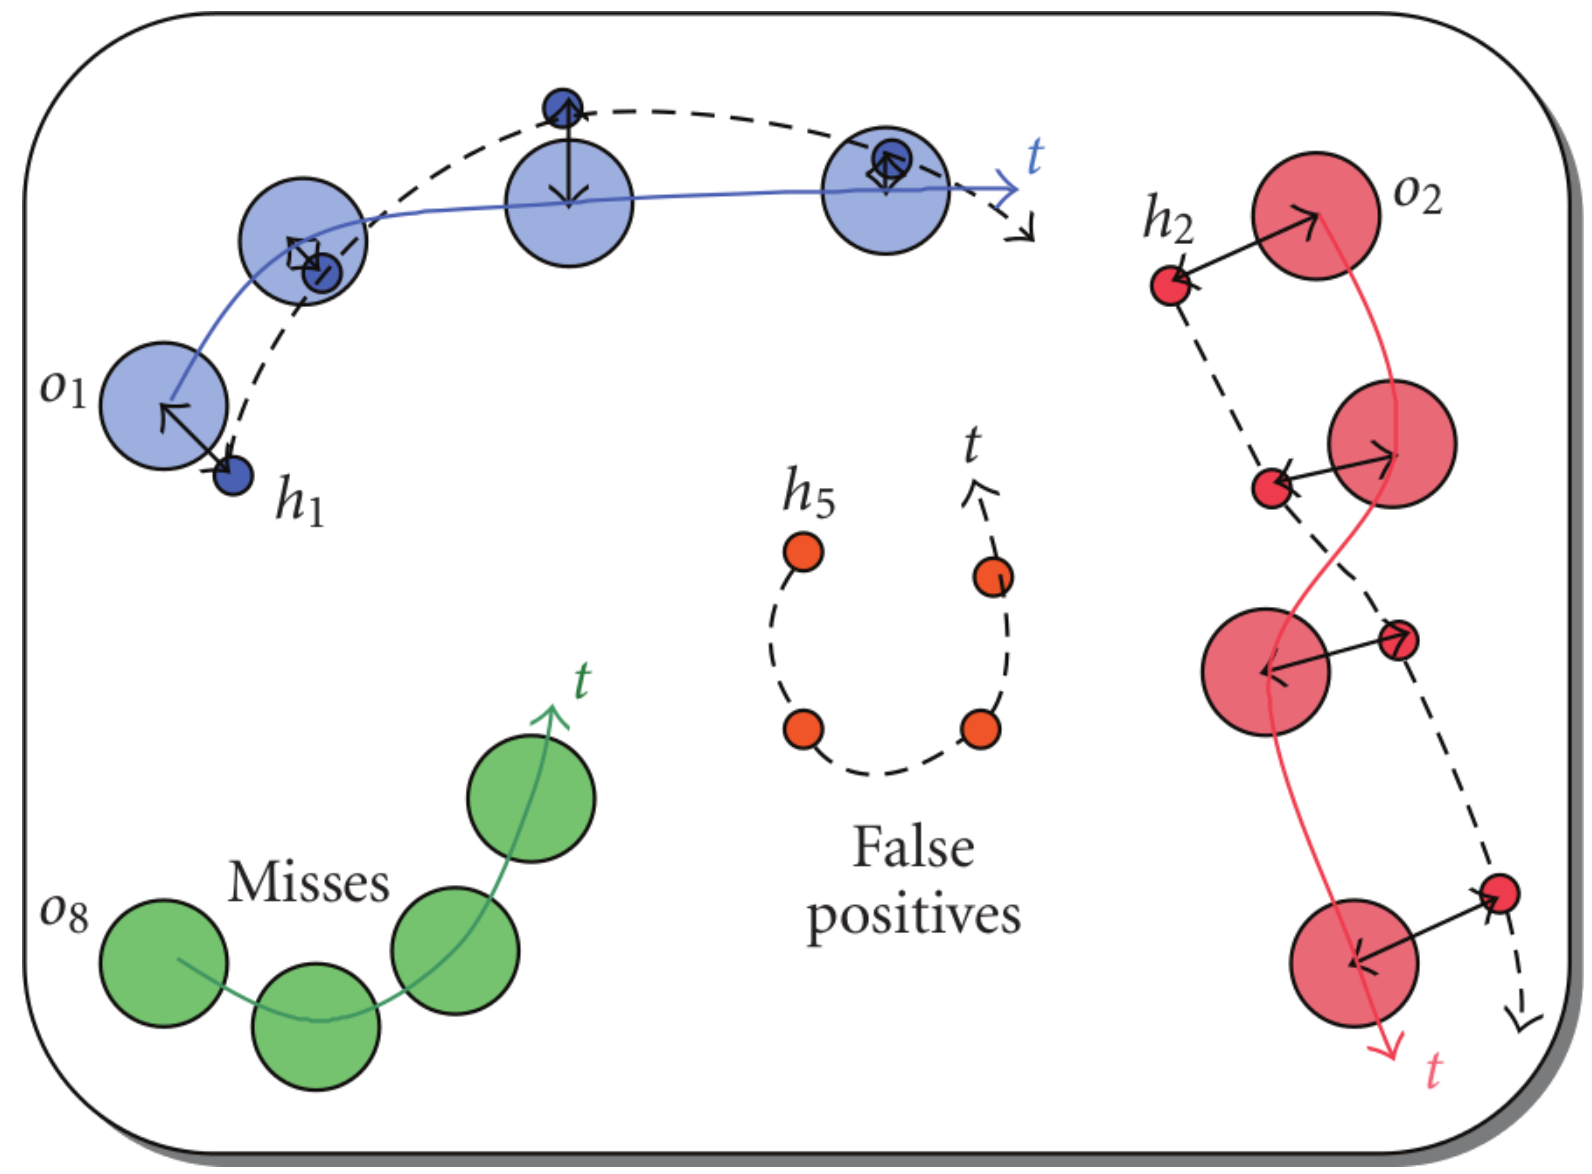
\includegraphics[width=120pt]{pics/fig2.png}
        \caption{TP's, FP's, FN's in consecutive frames.}
    \end{figure}

\end{frame}

\begin{frame}
    \frametitle{IDSW in Consecutive Frames}

    An {\bf IDSW (id switch)} event means there exist TP pairs, say $(g_i, p_j)\in\Pi^{(f)}$,
    $(g_k, p_\ell)\in\Pi^{(f+1)}$, in two consecutive frames
    $f$ and $f+1$ that satisfy
    \[
        \text{gtId}(g_i) = \text{gtId}(g_k),\ 
        \text{prId}(p_j) \neq \text{gtId}(p_\ell).
    \]
    Actually, this is an \emph{id mismatch} occuring in frame $f+1$.
    If two objects exchange their ids in new frame, then this is regarded as $2$
    IDSW events.
    \begin{figure}
        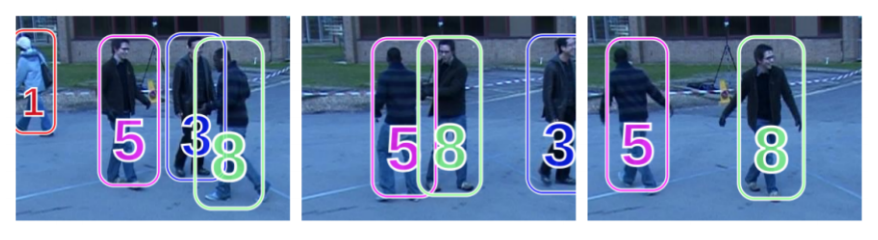
\includegraphics[width=180pt]{pics/fig3.png}
        \caption{The ids 3 \& 8 exchanges. 2 IDSW events.}
    \end{figure}
    
    
\end{frame}

\begin{frame}
    \frametitle{Matching in Sequence-Levels}
    
    Matchings in sequence-levels are done by associating one ground-truth trajectory
    % ({\tt gtTraj})
    to exactly one hypothetical trajectory
    % ({\tt prTraj})
    along a sequence of frames.
    Denote such matchings by $\mathfrak P$ (swash font).
    
    \quad

    % The similarity of a {\tt grTraj} and a {\tt prTraj} is often divided into
    % different levels: `mostly tracked' and `mostly lost'.
    Note that \emph{the similarities of two trajectories still depend on the
    framewise matching under some threshold.}
    When most objects are matched, then we call it `mostly tracked';
    Otherwise, we call it `mostly lost'.
    % Here it is usually defined in a Jaccard index (IoU) way:
    % \[
    %     \mathcal S_{\rm tr}(\text{\scriptsize gtTraj}, \text{\scriptsize prTraj}, \Pi_\alpha) =
    %         |\text{TP}| / (|\text{TP}|+|\text{FN}|+|\text{FP}|).
    % \]
    \begin{figure}
        \begin{subfigure}{.5\textwidth}
            \centering
            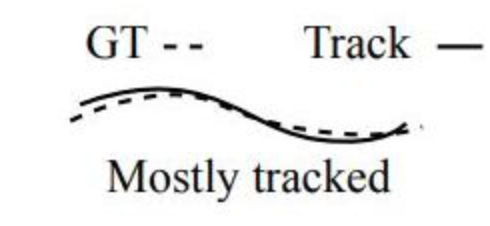
\includegraphics[width=80pt]{pics/fig4.png}
        \end{subfigure}%
        \begin{subfigure}{.5\textwidth}
            \centering
            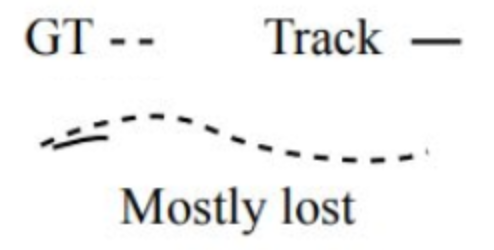
\includegraphics[width=70pt]{pics/fig5.png}
        \end{subfigure}
        \caption{Mostly tracked \& mostly lost.}
    \end{figure}

\end{frame}


\begin{frame}
    \frametitle{IDTP, IDFP and IDFN}

    Once if the trajectories are matched and denote the matching by $\mathfrak P$,
    we can define the performance measures as follows.

    \quad 

    Let $\alpha$ be a (detection-) similarity threshold.
    \begin{itemize}
    \item IDTP:
        the overlapping part (objects with $\mathcal S\geq \alpha$) of
        all $(\text{gtTr}, \text{prTr})\in\mathfrak P$.
        \[
            \text{IDTP} := 
                \left\{~(g,p)\ \left|\ 
                \begin{array}{l}
                g\in\text{gtTr},~ p\in\text{prTr},~ f_g = f_p, \\
                \mathcal S(g,p)\geq\alpha, \\
                \forall\ (\text{grTr}, \text{prTr})\in\mathfrak P.
                \end{array}
                \right.
                \right\}.
        \]
    \end{itemize}
    
\end{frame}

\begin{frame}
    \frametitle{IDTP, IDFP and IDFN}
    
    \begin{itemize}
    \item IDFP:
        non-matched predictions in matched pairs
        and all predictions in non-matched hypothetical trajectories.
        \begin{align*}
            \text{IDFP} := &
                \left\{~p \in \text{prDets}\ \left|\ 
                \begin{array}{l}
                \exists\ g\in\text{gtTr}^{(f_p)} ~ \suchthat ~
                \mathcal S(g,p) < \alpha, \\
                \text{or} ~ \text{gtTr}^{(f_p)} = \emptyset\ \\
                \forall\ (\text{gtTr}, \text{prTr}(p))\in\mathfrak P
                \end{array}
                \right.
                \right\}. \\
                & \bigcup \Big\{ ~p \in \text{prDets}\ |\ \text{{prTr}$(p)$ is not matched}.\Big\}
        \end{align*}
    \item IDFN:
        non-matched ground-truths in matched {gtTraj}'s and all ground-truths
        in non-matched {gtTraj}'s.
    \end{itemize}
\end{frame}

\begin{frame}
    \frametitle{Measures for Associations}

    By the concepts of matching in sequence-levels, we can further develop the
    measures for {\bf tracking associations} of an single object with ground-truths
    and predictions among all the matched trajectories.

    \quad 

    Let $c = (g,p)$ be a TP pair in some frame $t$. We can define the true positive
    associations by:
    \begin{align*}
        \text{TPA}(c) := 
            \left\{(g_i, p_j)\in\text{TP}\ \left|\ 
            \begin{array}{c}
                \text{grId}(g_i)=\text{grId}(g), \\
                \text{prId}(p_j) = \text{prId}(p)
            \end{array}\right.
            \right\}.
    \end{align*}
    Note that $|\text{TPA}(c)|$ is just the number of frames that $\text{gtTraj}(g)$
    and $\text{prTraj}(p)$ overlap.

\end{frame}

\begin{frame}
    \frametitle{Measures for Associations}

    Similarly, for the TP pair $c = (g, p)$, we also define the false positive associations
    and false negative associations as follows.
    \begin{align*}
        \text{FPA}(c) := &
            \left\{(g_i, p_j)\in\text{TP}\ \left|\ 
            \begin{array}{c}
                \text{grId}(g_i) \neq \text{grId}(g), \\
                \text{prId}(p_j) = \text{prId}(p)
            \end{array}\right.
            \right\} \\
            & ~ \bigcup ~
            \Big\{p_j\in\text{FP}\ |\ 
                \text{prId}(p_j) = \text{prId}(p)
            \Big\}; \\
        \text{FNA}(c) := &
            \left\{(g_i, p_j)\in\text{TP}\ \left|\ 
            \begin{array}{c}
                \text{grId}(g_i) = \text{grId}(g), \\
                \text{prId}(p_j) \neq \text{prId}(p)
            \end{array}\right.
            \right\} \\
            & ~ \bigcup ~
            \Big\{g_i\in\text{FN}\ |\ 
                \text{gtId}(g_i) = \text{gtId}(g)
            \Big\}.
    \end{align*}
    Note that $\text{FPA}(c)$ and $\text{FNA}(c)$ relate to the non-matched or id-mismatched
    objects in $\text{prTraj}(p)$ and $\text{grTraj}(g)$.

\end{frame}

\section{Metrics for Measuring Tracking Results}

\begin{frame}
    \frametitle{Metrics for Measuring Tracking Results}

    Performance of object trackings is based on the result of detections.

    \quad 

    To measure the results, the metrics often consists of the following aspects
    \begin{itemize}
    \item detection;%: measure accuracies of predictions
    \item localization;%: measure accuracies of positions of correct predictions
    \item association.%: measure accuracies of the correct associations of objects
    \end{itemize}
    
\end{frame}

\subsection{CLEAR-MOT}

\begin{frame}
    \frametitle{CLEAR-MOT: MOTA and MOTP}

    % {\scriptsize\tt K. Bernardin \& R. Stiefelhagen, Evaluating Multiple Object Tracking Performance:%
    % The CLEAR MOT Metrics.}

    Given a similarity threshold $\alpha$.

    \quad

    {\bf MOTA (multiple object tracking accuracy)} is calculated through optimizing the value
    \[
        \text{MOTA}_\alpha :=
            \max_{\Pi_\alpha}
            \left\{1 - \dfrac{|\text{FN}_{\Pi_\alpha}| + |\text{FP}_{\Pi_\alpha}| + |\text{IDSW}_{\Pi_\alpha}|}{|\text{gtDet}|}\right\}
    \]
    among all matchings $\Pi_\alpha$ with $\mathcal S(c)\geq \alpha$ for all matched $c\in\Pi_\alpha$.

    \quad

    Note that here the matching is done in frame-levels.
    This value measures the accuracy of detections by FN's and FP's;
    and the accuracy of id-associations by IDSW's.

\end{frame}

\begin{frame}
    \frametitle{CLEAR-MOT: MOTA and MOTP}

    As MOTA is achieved by some matching $\Pi_\alpha$, {\bf MOTP (multiple object tracking precision)}
    is calculated as follows:
    \[
        \text{MOTP}_\alpha =
            \dfrac{\sum_{(g,p)\in\text{TP}_{\Pi_\alpha}}\mathcal S(g,p)}{|\text{TP}_{\Pi_\alpha}|}.
    \]

    \quad 

    Note that this measures the accuracy of tracking associations.

\end{frame}

\subsection{Performance Measures for MTMCT}

\begin{frame}
    \frametitle{ID-Precision, ID-Recall, IDF1 for MTMCT}

    As a measure for the {\bf MTMCT (multi-target, multi-camera tracking)} tasks,
    the id metrics focus on matching of trajectories.

    \quad 

    Under a similarity threshold $\alpha$, the scoring functions are calculated through optimizing
    the quantity $|\text{IDTP}|$ by matching as follows:
    \begin{align*}
        \text{ID-Precision} := & ~ \dfrac{|\text{IDTP}|}{|\text{IDTP}| + |\text{IDFP}|}, \\
        \text{ID-Recall} := & ~ \dfrac{|\text{IDTP}|}{|\text{IDTP}| + |\text{IDFN}|}, \\
        \text{IDF1} := & 
            ~ \dfrac{|\text{IDTP}|}{|\text{IDTP}| + 0.5|\text{IDFP}| + 0.5|\text{IDFN}|}.
    \end{align*}

\end{frame}

\end{document}